% Old Rows 3-4 (setup, key result, benchmarks, ablation, robust & efficient), replaced by the
% single Experiments box. To restore a piece, copy it back into blade-poster.tex.
      % ======================= Row 3: experiments + key result =======================
      \begin{columns}[T]
        \begin{column}{0.40\linewidth}
          \begin{psublock}[equal height group=r3]{Experimental setup}
            \begin{columns}[T]
              \begin{column}{0.325\linewidth}
                \begin{benchtile}{\faIcon{user-friends}\ TOFU\autocite{maini2024tofu}}
                  \small synthetic authors\\
                  forget 1/5/10\%\\[0.4ex]
                  \textbf{Llama-3.2 1B/3B}
                \end{benchtile}
              \end{column}
              \begin{column}{0.325\linewidth}
                \begin{benchtile}{\faBook\,\faNewspaper\ MUSE\autocite{shi2025muse}}
                  \small Books (Harry Potter)\\
                  News (BBC)\\[0.4ex]
                  \textbf{Llama-2-7B}
                \end{benchtile}
              \end{column}
              \begin{column}{0.325\linewidth}
                \begin{benchtile}{\faCopyright\,\faIcon{user-lock}\ KnowUndo\autocite{tian2024knowundo}}
                  \small copyright\\
                  privacy\\[0.4ex]
                  \textbf{Llama-2-7B-chat}
                \end{benchtile}
              \end{column}
            \end{columns}
            \vspace{1ex}
            \textbf{Baselines:}
            \chip{GradAscent\autocite{jang2023knowledge}} \chip{GradDiff} \chip{NPO\autocite{zhang2024negative}} \chip{SimNPO\autocite{fan2025simplicity}} \chip{RMU} \chip{BLURNPO} \chip{PDU}\\[0.8ex]
            \textbf{Metrics:} HM of forget \& retain axes · LLM judge HM$_\text{J}$ · 5 seeds
          \end{psublock}
        \end{column}
        \begin{column}{0.58\linewidth}
          \begin{psublock}[colframe=psu-navy, colbacktitle=psu-navy, boxrule=5pt, equal height group=r3]%
            {{Key result: stable under scaling and repeated unlearning}}
            \begin{columns}[c]
              \begin{column}{0.56\linewidth}
                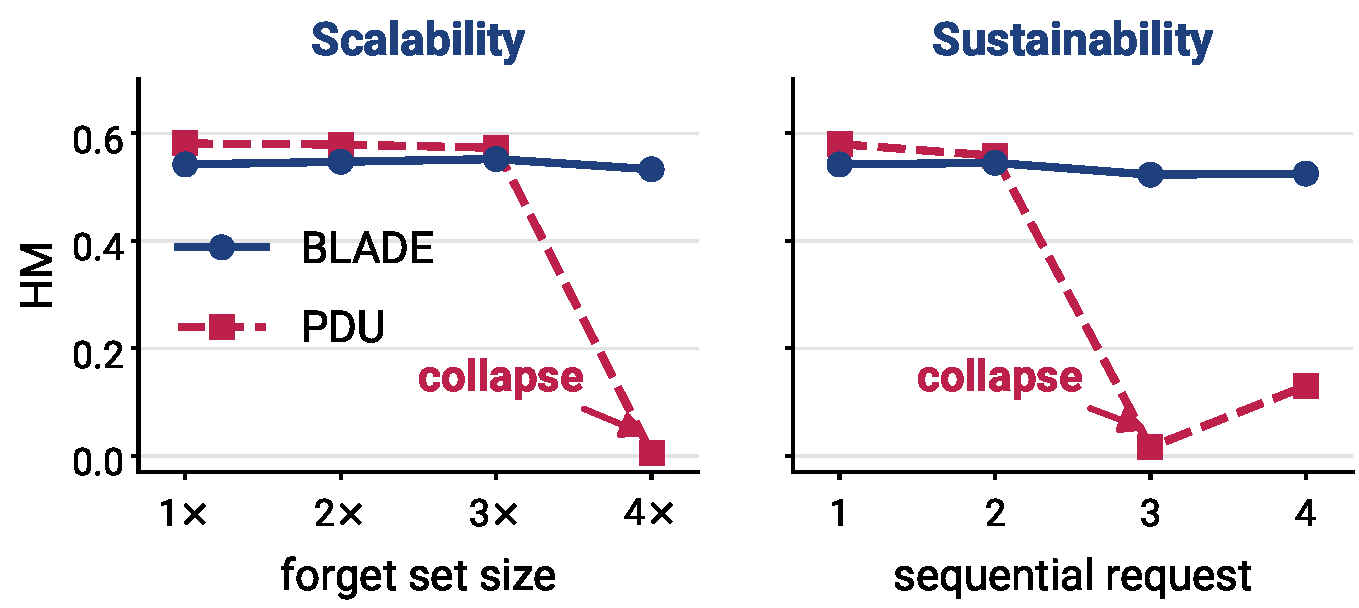
\includegraphics[width=\linewidth]{figures/fig_stress}
              \end{column}
              \begin{column}{0.42\linewidth}
                \raggedright
                \bignum{psu-pink}{0.58 $\to$ 0.005}{PDU at $4\times$ forget set}
                \bignum{psu-pink}{0.58 $\to$ 0.02}{PDU after 2 sequential steps}
                \bignum{psu-beaver}{0.52--0.55}{\method HM, every condition}
              \end{column}
            \end{columns}
            \vspace{0.4ex}
            \centering{\small MUSE News · PDU\autocite{entesari2026constrained} = strongest News baseline}\\[0.4ex]
            \textbf{Why:} \circnum{3} bounded loss · LoRA bottleneck · \circnum{2} ALM ratchet
          \end{psublock}
        \end{column}
      \end{columns}

      % ======================= Row 4: supporting results =======================
      \begin{columns}[T]
        \begin{column}{0.46\linewidth}
          \begin{psublock}[equal height group=r4]{Best on three benchmark families}
            \centering
            {\LARGE\bfseries\color{psu-beaver}+6\%}\ TOFU \qquad
            {\LARGE\bfseries\color{psu-beaver}+9\%}\ MUSE Books \qquad
            {\LARGE\bfseries\color{psu-beaver}+7\%}\ KnowUndo\\[0.2ex]
            {\small average composite score vs.\ strongest baseline \quad {\color{psu-black!45}\faCircle[regular]}~best baseline \ {\color{psu-beaver}\faCircle}~\method}\\[0.6ex]
            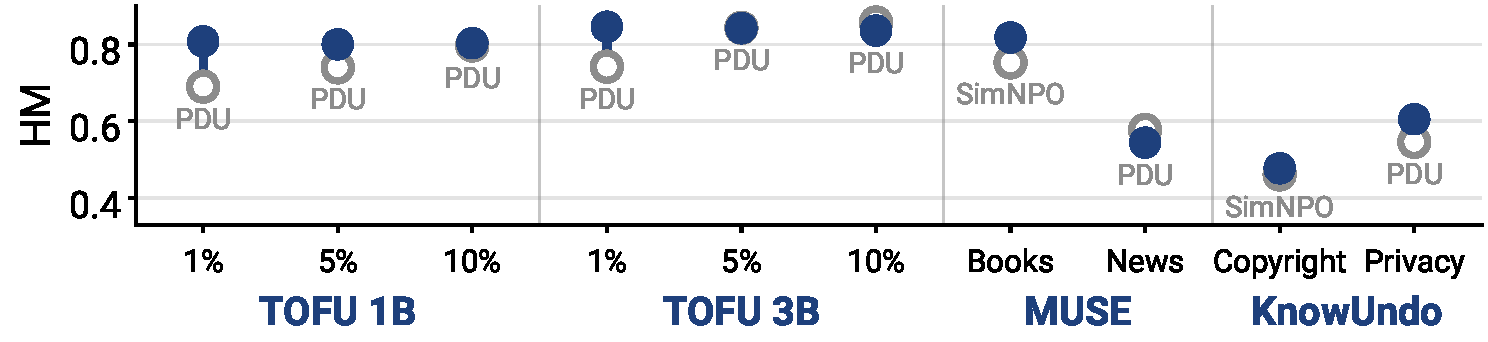
\includegraphics[width=\linewidth]{figures/fig_benchmarks}\\[0.4ex]
            LLM judge: \method best HM$_\text{J}$ on \textbf{6 of 7} settings
          \end{psublock}
        \end{column}
        \begin{column}{0.28\linewidth}
          \begin{psublock}[equal height group=r4]{Every component matters}
            \centering{\small MUSE Books HM, one change at a time}\\[0.8ex]
            \adjustbox{max width=\linewidth}{% Ablation on MUSE Books (HM, higher is better; paper ablation table): one design change per row.
% Row labels carry the component number they ablate.
\begin{tikzpicture}[x=11cm, y=-1.65cm]
  \foreach \i/\name/\v/\c in {%
      0/Full \textbf{BLADE}/0.823/psu-beaver,
      1/\circnum{2} ALM off/0.233/psu-pink,
      2/no LoRA (full FT)/0.459/psu-pink,
      3/\circnum{1} loops swapped/0.506/psu-pink,
      4/\circnum{3} unclamped ($\tau{=}1$)/0.780/psu-pink,
      5/\circnum{3} GA loss instead/0.160/psu-pink,
      6/\circnum{3} NPO loss instead/0.009/psu-pink} {
    \node[anchor=east, inner sep=10pt] at (0,\i) {\name};
    \fill[\c] (0,\i-0.3) rectangle (\v,\i+0.3);
    \node[anchor=west, inner sep=8pt, font=\bfseries, text=\c] at (\v,\i) {\v};
  }
  \draw[line width=2pt, psu-navy] (0,-0.5) -- (0,6.5);
\end{tikzpicture}
}
          \end{psublock}
        \end{column}
        \begin{column}{0.24\linewidth}
          \begin{psublock}[equal height group=r4]{{Robust and efficient}}
            \raggedright
            \setlength{\tabcolsep}{4pt}\renewcommand{\arraystretch}{1.5}
            \begin{tabular}{@{}c@{\ \ }p{0.8\linewidth}@{}}
              {\Large\color{psu-beaver}\faSearch} & \textbf{Extraction:} best adv.\ HM \\
              {\Large\color{psu-beaver}\faIcon{user-secret}} & \textbf{Jailbreak:} lowest ASR \\
              {\Large\color{psu-beaver}\faIcon{user-shield}} & \textbf{MIA:} no leakage \\
              {\Large\color{psu-beaver}\faTerminal} & \textbf{GCG:} lowest ASR (fgt01) \\
              {\Large\color{psu-beaver}\faMemory} & \textbf{2--5$\times$ less} GPU memory \\
            \end{tabular}\\[0.4ex]
            {\small attacks: TOFU, Llama-3.2-1B}
          \end{psublock}
        \end{column}
      \end{columns}

